\section{Realtime planlægning i \pycsp}
\label{sec:rtp-pycsp}
\fxnote{(Flyttet fra RTP overordnet) Husk at snakke om begrænsning af greenlets mht. parallelitet når vi arbejder i realtid}
Da vi ønsker at introducere RTP i \pycsp, er der er række forhold, som vi skal tage højde for. Vi vil i dette afsnit tage udgangspunkt i de ovenstående opstillede muligheder og sammenholde dem med \pycsp. 

I \pycsp kan vi anskue processerne som begivenheder og derved bruge skemaplanlæggeren i \code{greenlets}-versionen til at styre hvilken proces og dermed hvilken begivenhed, der udføres. Vi har ikke umiddelbart informationer om, hvor lang tid en proces er om at blive udført, og det vil kræve en analyse af den enkelte proces at udlede estimater for det. Vi har valgt at fokusere på selve planlægningen af processerne og ikke på analysen. Dermed har vi ikke mulighed for at benytte RM og LL algoritmerne, da de begge benytter information om udførselstiden for en proces. Derved har vi EDF tilbage som mulighed, hvilket vi i det følgende vil implementere. En udvidelse af \pycsp til at benytte EDF er forholdsvis ligetil. Der skal laves en mulighed for, at brugeren kan angive en deadline til en proces, og vi skal ved kontekstskift sikre, at vi aktiverer den proces, der har den førstkomne deadline. Såfremt en deadline overskrides, skal vi have funktionalitet, til at håndtere dette. 

\pycsp har per definition interne afhængigheder mellem processerne i form af kommunikation over kanaler, og vi kan derfor opleve problemer med prioritetsinvertering. Den eneste metode til håndtering af dette, der kan bruges sammen med \pycsp, er prioritetsnedarvning, da de andre metoder forudsætter prioritetsinverteringen  sker som resultat af tilgang til kritiske regioner og ikke pga. kommunikation. Vi skal derfor også implementere prioritetsnedarvning for at sikre os mod prioritetsinvertering. 

Da vi benytter os af \code{greenlets}-versionen af \pycsp arbejder vi med en skemaplanlægger, der ikke kan foretage preemptive kontekstskift. Dette kan lede til problemstillinger som det er illustreret på \cref{fig:edf-nonpreemptive}. En metode til at mindske denne type problemer er at lade de enkelte processer afgive kontrollen med jævne mellemrum. Herved vil der blive foretaget en ny evaluering om hvilken proces, der skal aktiveres, og hvis der er processer, der har en nærmere deadline, som er blevet klar, aktiveres en af disse. Dette beror helt og holdent på at hver enkelt proces frivilligt afgiver kontrollen og gør det med jævne mellemrum, når den er aktiv. Dette betyder, at det er overladt til udvikleren at indsætte det på relevante steder i processens kode. 

\subsection{Tilknytning og overskridelse af deadlines}
Som udgangspunkt skal vi kunne håndtere, at en proces kan have forskellige typer deadlines. Umiddelbart er det oplagt, at der for hver proces tilknyttes en deadline samt hvilken type, det er. Dette giver mulighed for, at vi kan differentiere i den måde vi håndterer en overskreden deadline. F.eks. kan vi stoppe systemet helt i tilfælde af overskridelse af en kritisk deadline, kaste en exception ved en hard deadline og blot registrere overskridelser af soft deadlines. Uanset hvilken handling vi vælger at tilknytte til de respektive overskridelser, vil der altid være situationer, hvor den valgte handling ikke er optimal. 

Vi har derfor valgt en anden løsning, hvor en proces blot kaster en exception, hvis den overskrider en deadline. Dette overflødiggør, at der tilknyttes en specifik type deadline til en proces, da håndteringen af den kastede exception overgives til udvikleren. Det er herved op til den enkelte udvikler at definere, hvad der skal ske i hver enkelt proces, såfremt den overskrider en deadline. Dette giver den største frihed til at tilpasse håndteringen til den enkelte proces og applikation. 

\subsection{Udvælgelse af proces}
Udvælgelsen af hvilken proces der skal aktiveres, ved et kontekstskift, er givet ud fra vores valg af EDF. Som beskrevet i \cref{sec:edf} specificerer EDF, at det altid processen med den nærmeste deadline der skal aktiveres. For at opnå dette kan vi benytte stort set samme metode som vi brugte i \des. I \des sorterede vi processerne efter hvilket tidskridt de skulle aktiveres i, her kan vi sortere dem ud fra deres deadline.  

\subsection{Kommunikation}
I litteraturen for  RTP fokuseres der kun på udvælgelsen og planlægningen af processer i \sched en. I \pycsp er det ikke kun  \sched en der bestemmer om en proces kan eksekveres, men er også afhængig af at kunne kommunikere over kanalerne. Dette er ikke et problem ved one-to-one kanaler, hvor der kun er en proces i hver ende, og processen dermed er garanteret at gennemføre kommunikationen hvis modparten er klar til at kommunikere. I \pycsp er one-to-one kanalerne blevet fjernet, og erstattet af any-to-any kanaler. Ud fra et teknisk synspunkt er disse mere generelle og kan alt som one-to-one kanalerne kan. Dette er dog ikke optimalt i forbindelse med RTP, da der til hver af kanalerne kan være et vilkårligt antal processer der ønsker at sende og modtage data på et givent tidspunkt. I one-to-one kanalerne kan man  umiddelbart foretage kommunikationen når der findes to processer der ønsker at kommunikere. I any-to-any kanalerne kan der være flere processer i den samme kanal, der venter på en proces der ønsker at kommunikere. Når der ankommer en proces der ønsker at kommunikere kan kun en af de ventende processer fuldføre sin kommunikation. I \pycsp foregår denne parring mellem processer tilfældigt, og kan derfor resultere i at processer med en lav prioritet foretager kommunikationen før en højt prioriteret proces. Når processer kommunikere i RTP i any-to-any kanaler, kan man med fordel sikre at det altid kommer til at foregå mellem de to processer der har den højeste prioritet.

\subsubsection{Kommunikation i \code{alternations}}
Det er dog ikke kun i forbindelse med blokerende kommunikation vi skal forholde os til introduktionen af processer med  prioritet. I kodestrukturen \code{alternation}
 har en udvikler mulighed for at foretage et  prioriteret valg mellem flere forskellige kanaler. Et prioriteret valg mellem flere kanaler, kan dog være i konflikt med de processernes prioritet. 
  
\citeauthor{Burns1990} beskriver præcist denne problemstilling\cite{Burns1990}. Til at illustrere problemet beskriver de et eksempel, som er vist i \cref{lst:pri-select}. Denne kodestump viser et prioriteret valg mellem kanalerne A1 og A2. Til hver kanal er tilknyttet en proces, P1 og P2. Disse to processer har en prioritet tilknyttet på hhv.  Pri1 og Pri2. \CRef{tab:prioritizedSelect} viser resultatet af dette valg, afhængig af prioriteternes indbyrdes forhold.


\begin{lstlisting}[firstnumber=1 ,float=hbtp, label=lst:pri-select, caption={(priority) select. Eksemplet er kopieret fra \cite{Burns1990}}]
(priority) select
   A1 -- Process P1
 or
   A2 -- Process P2
 end select
\end{lstlisting}

\begin{table}[htbp]
	\centering
	\begin{tabular}{lccc}
       	\toprule
        &Pri1 > Pri2 & Pri1 = Pri2 & Pri1 < Pri2\\
        \midrule
		    priority select & A1 & A1           & ?  \\
        \bottomrule
        \end{tabular}
    \caption[]{Konflikten ved brug af prioriteret valg og procesprioriteter. Eksemplet er kopieret fra \cite[160]{Burns1990}}\\
    \label{tab:prioritizedSelect}
\end{table}

MANGLER MERE HERRRRR\\
\cref{tab:prioritizedSelect} og konstatere, at der opstår en konflikt ved introduktionen af prioriteter. For \citeauthor{Burns1990} er løsningen ``orthogonal solutions'', der håndterer begge typer prioriteter. De ønsker overordnet set to typer udvælgelsesmetoder, weak- og strong Select. Weak select sorterer primært efter processernes prioritet og sekundært efter det prioriterede valg. Strong select udvælger udelukkende processer efter det prioriterede valg. De forestiller sig, at weak select skal bruges som den primære metode, men i specielle tilfælde skal en udvikler have mulighed for at tvinge et prioriteret valg igennem.

Vi ønsker at udvælgelse i \code{alternations} udføres som weak select. Dvs. at først skal der kigges på, om \code{alternation} kan vælge en guard umiddelbart. Hvis der er minimum en guard klar, foretages der et prioriteret valg baseret på processernes prioritet. Hvis flere processer har samme prioritet foretages det prioriterede valg. Er ingen guards klar, bør processen vente i dens \code{alternation}, og vælge den første guard, der bliver klar, uden hensyn til dens prioritet.

I artiklen fra \citeauthor{Burns1990} udvælger man en proces blandt flere mulige, mens en \code{alternation} udvælger en kanal, der i \pycsp er af typen any-to-any. Dette medfører, at man ikke  foretager et valg mellem processer, men foretager et valg mellem kanaler, som processen kommunikerer med. For at foretage en weak selection i vores \code{alternation}, skal man derfor kunne finde prioriteten for kanalerne. Dette skaber et behov for at kunne tilknytte en prioritet til hver kanal baseret på hvilke processer, der er tilknyttet kanalen. 
\phantomsection
\label{misc:kanal-prioritet}


\subsection{Prioritetsnedarvning}\label{sec:rtp-pycsp-nedarvning}
At introducere prioritetsnedarvning i \pycsp virker umiddelbart ligetil, idet vi kan se de indbyrdes afhængigheder klart ud fra forbindelserne gennem kanalerne. Der kan forekomme andre afhængigheder, som er mindre synlige, men vi mener ikke disse vil forekomme i velskrevne CSP applikationer, og vi har derfor valgt at begrænse os til afhængigheder repræsenteret vha. kanaler. På trods af den umiddelbare simplicitet skal vi overveje hvornår, hvem og hvor længe, der skal arves i forbindelse med prioritetsnedarvning.

\subsubsection*{Ændring af prioritet}
\label{sec:aendring-af-prioritet}
Vi arbejder med et dynamisk system af processer, hvor en proces, på baggrund af sin tilstand, er afhængig af forskellige andre processer for at kunne arbejde videre. 
Hvis vi højner prioriteten på alle processer, der er forbundet til en proces med høj prioritet, vil mange af processerne, der arver den høje prioritet, reelt ikke kunne bidrage til udførelsen af den proces, der starter med høj prioritet. Det er en bedre løsning, at det kun er den eller de processer, der kan sikre videre udførsel af den aktuelle proces, der tildeles højere prioritet. Hvis eksempelvis en proces med høj prioritet ønsker at skrive på en kanal, skal alle processer, der læser på den kanal, arve den høje prioritet, men de processer, som ønsker at skrive til en anden kanal, som processen med høj prioritet læser fra, skal ikke arve den høje prioritet. Generelt set betyder det, at der kun skal udføres prioritetsnedarvning, såfremt en højt prioriteret proces venter på at kommunikere, uden der er andre processer, der er klar til at indgå i den ønskede kommunikation. 

Vi har nu begrænset os til, at det kun er de processer der kan indgå i kommunikation over en kanal, der arver en prioritet. Med any-to-any kanaler findes der dog et vilkårligt antal processer i hver kanalende, og man risikerer en prioritetsdevaluering ved at lade flere processer arve en høj prioritet. I klassisk \csp findes der modsat hertil one-to-one kanaler, hvor man er sikret at det kun én proces' prioritet der bliver højnet ved prioritetsnedarvning. Forskellen kan illustreres af \autoref{fig:one-to-one-inheritance} og \cref{fig:any-to-any-inheritance}\fxwarning{tjek sidenr. er korrekt for de to figurer inden aflevering}. På \autoref{fig:one-to-one-inheritance}, bliver en proces' prioritet hævet fra fem til 10. Modtageren kan uden afbrydelser arbejde hen mod at kunne kommunikere, da afsenderen venter. I \autoref{fig:any-to-any-inheritance} bliver alle tre processers prioritet hævet til 10 og de vil skulle kæmpe mod hinanden for komme frem til en tilstand hvor de ønsker at kommunikere. 

\begin{figure}
 \begin{center}
  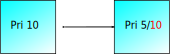
\includegraphics[scale=1.00]{images/one-to-one-inheritance}
\caption{Procesnetværk med en afsender og en modtager. Afsenderen har prioritet 10, mens modtageren har en initiel prioritet på fem. Modtageren  får via prioritetsnedarvning hævet sin prioritet til 10. (Højere er bedre)}
  \label{fig:one-to-one-inheritance}
  \end{center}
\end{figure}

\begin{figure}
 \begin{center}
  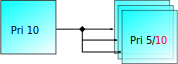
\includegraphics[scale=1.00]{images/any-to-any-inheritance}
  \caption{I dette eksempel findes der tre modtagere, som alle får hævet deres prioritet til 10.}
  \label{fig:any-to-any-inheritance}
  \end{center}
\end{figure}

 Prioritetsnedarvning i et miljø med any-to-any kanaler har dermed en risiko for at medføre prioritetsdevaluering. Man kan forstille sig forskellige metoder til at eliminere eller minimere problemet f.eks ved at begrænse antallet af processer, der kan modtage en prioritetsnedarvning. Dette kunne gøres ved kun at lade en enkelt proces arve prioriteten,  men så skal man tage stilling til, hvilken proces, der skal udvælges. Dette kunne være den proces, der er tættest på at indgå i kommunikationen.  Udvælgelsen af processer må dog bero på en analyse af den enkelte applikation og dens aktuelle tilstand. Da vi ikke ønsker at begynde på en analyse af brugerens kode, må vi nødvendigvis sende prioritetsnedarvningen til alle processerne på kanalen. For at løse problemet vil vi i stedet fokusere på at minimere antallet af processer, der starter prioritetsnedarvningen, og det tidsrum processerne har arvet en prioritet.

Når kommunikationen på kanalen er gennemført, befinder processens sig i en anden tilstand og er afhængig af noget andet for at komme videre i sin udførsel. 
Når det midlertidige afhængighedsforhold ophører skal processer der har arvet en prioritet miste denne. Der skal selvfølgelig tages højde for at en proces kan arve forskellige prioriteter fra forskellige andre processer, så det skal være muligt at falde tilbage til den næsthøjeste arvede prioritet, i stedet for blot at skifte tilbage til den oprindelige prioritet. 

\subsubsection*{Prioritetsnedarvning i \code{alternations}}
Vi har som nævnt en klar kæde af afhængigheder i \pycsp men vi skal være opmærksomme på ikke at højne processers prioritet unødigt. Dette kan let blive tilfældet såfremt vi ikke holder ordentligt styr på, hvorfor en proces har den prioritet, den har, om den er sat af udvikleren, eller den er nedarvet. Man kan forestille sig en situation, hvor et uddrag af et proces-neværk består af en generator-forbruger-model med to generatorer og en enkelt forbruger. De to generatorer er forbundet til forbrugeren vha. en \code{alternation}, og har henholdsvis høj og lav prioritet. Eksemplet er illustreret på \cref{fig:alt-inheritance}. Forbrugeren vil i dette scenarium arve den høje prioritet fra den tilsvarende generator, men utilsigtet vil den høje prioritet derefter også propagere fra forbrugeren til generatoren med lav prioritet. Dette er ikke hensigtsmæssigt, da de to generatorer nu har lige høj prioritet og ikke det forhold, som udvikleren oprindeligt har angivet. Vi kan dog indse, at dette ikke bliver et problem, idet vi kun udfører prioritetsnedarvning i det tilfælde, hvor der ikke er nogen processer, der er er klar til at indgå i ønsket kommunikation. I det opstillede tilfælde vil forbrugeren derfor ikke foretage yderligere prioritetsnedarvning på generatoren med lav prioritet, da generatoren med høj prioritet altid vil være klar til at skrive i denne situation. 

\begin{figure}
 \begin{center}
  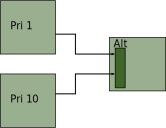
\includegraphics[scale=1.00]{images/alt-inheritance}
  \caption{Prioritetsnedarvning i \code{alternations.}}
  \label{fig:alt-inheritance}
  \end{center}
\end{figure}
